\documentclass[11pt,a4paper]{article}

\usepackage[margin=1in]{geometry}
\usepackage{mathptmx}
\usepackage{amsmath}
\usepackage{amssymb}
\usepackage{amsthm}
\usepackage{braket}
\usepackage{tikz}
\usetikzlibrary{shapes.geometric}
\usepackage{quantikz}
\usepackage{enumitem}
\usepackage{hyperref}
\usepackage{xcolor}

\definecolor{circuitblue}{RGB}{40,80,160}

\hypersetup{
    colorlinks=true,
    linkcolor=circuitblue,
    urlcolor=circuitblue,
    citecolor=circuitblue
}

\theoremstyle{definition}
\newtheorem{definition}{Definition}[section]
\newtheorem{example}{Example}[section]
\newtheorem{theorem}{Theorem}[section]

\theoremstyle{remark}
\newtheorem*{intuition}{Intuition}
\newtheorem*{keypoint}{Key Point}

\pagestyle{plain}

\setlength{\parindent}{0pt}
\setlength{\parskip}{6pt}

\begin{document}

\begin{center}
    {\LARGE \textbf{Hardware Efficient Ansatze for QML}}\\[8pt]
    {\large QML}\\[12pt]
    \hrule
\end{center}

\vspace{12pt}
\tableofcontents
\newpage

%% ========================================================
\section{Overview}
%% ========================================================

last lecture we learned that real quantum hardware is noisy, has limited connectivity, and can only faithfully execute circuits up to a certain depth. this lecture is about wt u do about it: how to design variational ansatze that respect hardware constraints while still being expressive enough for QML.

the central tension is simple: u want ur ansatz to be expressive (so it can represent complex functions) but shallow (so noise doesnt destroy the signal). hardware-efficient ansatze try to get the maximum expressiveness per unit of circuit depth by using only gates that the hardware natively supports and only connections that exist in the physical qubit topology.

well cover the main hardware-efficient ansatz families (RealAmplitudes, EfficientSU2, TwoLocal), understand transpilation and how it affects circuit depth, and develop practical guidelines for choosing and designing ansatze for specific hardware.

the punchline: the ``best'' ansatz isnt the most expressive one --- its the one that gives the most useful expressiveness within ur noise budget.

%% ========================================================
\section{What Makes an Ansatz ``Hardware Efficient''?}
%% ========================================================

\begin{definition}[Hardware-Efficient Ansatz]
an ansatz $U(\theta)$ is hardware-efficient if:
\begin{enumerate}[label=(\arabic*)]
    \item it uses only gates from the hardware's native gate set
    \item it respects the hardware's qubit connectivity (entangling gates only between physically connected qubits)
    \item it minimizes circuit depth for a given number of parameters
\end{enumerate}
\end{definition}

why does this matter? bcs any gate thats not in the native gate set must be decomposed into native gates, adding depth. any entangling gate between non-connected qubits requires SWAP routing, adding even more depth. and every additional gate adds noise.

\begin{example}
suppose ur ideal ansatz uses a CNOT between qubits 0 and 5 on a heavy-hex lattice where the shortest path from $q_0$ to $q_5$ is 4 edges. u need 3 SWAP gates to bring the qubits adjacent, each SWAP costs 3 CNOTs, so that single logical CNOT becomes $3 \times 3 + 1 = 10$ physical CNOTs. if ur 2Q gate error is 0.5\%, that one ``gate'' now has error $\approx 1 - (1-0.005)^{10} \approx 4.9\%$. thats terrible.
\end{example}

\begin{keypoint}
a hardware-efficient ansatz avoids this blowup by construction. it only uses gates and connections that map directly to the hardware, so wt u design is (approximately) wt gets executed.
\end{keypoint}

%% ========================================================
\section{Native Gate Sets}
%% ========================================================

every quantum processor has a small set of gates it can physically implement. everything else gets decomposed into these native gates during transpilation.

\subsection{IBM Native Gates}

IBM's superconducting processors use the following native gate set:

\begin{center}
\renewcommand{\arraystretch}{1.4}
\begin{tabular}{|c|c|c|}
\hline
\textbf{Gate} & \textbf{Matrix} & \textbf{Type} \\
\hline
$R_z(\lambda)$ & $\begin{pmatrix} e^{-i\lambda/2} & 0 \\ 0 & e^{i\lambda/2} \end{pmatrix}$ & 1Q, virtual (zero error) \\
\hline
$\sqrt{X}$ (SX) & $\frac{1}{2}\begin{pmatrix} 1+i & 1-i \\ 1-i & 1+i \end{pmatrix}$ & 1Q, physical \\
\hline
$X$ & $\begin{pmatrix} 0 & 1 \\ 1 & 0 \end{pmatrix}$ & 1Q, physical \\
\hline
ECR & $\frac{1}{\sqrt{2}}\begin{pmatrix} 0 & 0 & 1 & i \\ 0 & 0 & i & 1 \\ 1 & -i & 0 & 0 \\ -i & 1 & 0 & 0 \end{pmatrix}$ & 2Q, physical \\
\hline
\end{tabular}
\end{center}

\begin{keypoint}
$R_z$ gates on IBM hardware r ``virtual'' --- they r implemented by adjusting the phase of subsequent pulses rather than applying a physical pulse. this means $R_z$ gates have essentially zero error and zero duration. design ur ansatze to use lots of $R_z$ and minimize physical gates (SX, ECR).
\end{keypoint}

\subsection{Google Native Gates}

Google's Sycamore processor uses:
\begin{itemize}[leftmargin=*]
    \item single-qubit: arbitrary $R_z(\theta)$, $\sqrt{W} = \frac{R_x(\pi/2) + R_y(\pi/2)}{\sqrt{2}}$
    \item two-qubit: $\sqrt{\text{iSWAP}}$ and SYC (Sycamore gate)
\end{itemize}

the Sycamore gate is:
\[
\text{SYC} = \text{fSim}\left(\frac{\pi}{2}, \frac{\pi}{6}\right) = \begin{pmatrix} 1 & 0 & 0 & 0 \\ 0 & 0 & -i & 0 \\ 0 & -i & 0 & 0 \\ 0 & 0 & 0 & e^{-i\pi/6} \end{pmatrix}
\]

\subsection{Trapped Ion Native Gates}

IonQ and Quantinuum use:
\begin{itemize}[leftmargin=*]
    \item single-qubit: $R(\theta, \phi) = \exp\left(-i\frac{\theta}{2}(\cos\phi \, \sigma_x + \sin\phi \, \sigma_y)\right)$ (arbitrary axis in XY plane)
    \item two-qubit: MS gate $\text{MS}(\theta) = \exp\left(-i\frac{\theta}{4}\sigma_x \otimes \sigma_x\right)$ (IonQ) or ZZ interaction (Quantinuum)
\end{itemize}

%% ========================================================
\section{Gate Decomposition}
%% ========================================================

when ur circuit uses gates that arent in the native set, the transpiler must decompose them. understanding these decompositions helps u estimate the true cost of ur ansatz.

\subsection{Single-Qubit Gate Decomposition}

any single-qubit unitary can be decomposed using the Euler decomposition:
\[
U = e^{i\alpha} R_z(\beta) R_y(\gamma) R_z(\delta)
\]

on IBM hardware, since $R_y(\gamma) = R_z(-\pi/2) \cdot \text{SX} \cdot R_z(\pi/2 - \gamma) \cdot \text{SX} \cdot R_z(\gamma - \pi)$ (approximately), any single-qubit gate costs at most 2 SX gates and 3 $R_z$ gates. since $R_z$ is virtual, the physical cost is just 2 SX gates.

\begin{example}
decomposing a Hadamard gate on IBM hardware:
\[
H = R_z(\pi) \cdot \text{SX} \cdot R_z(\pi)
\]
cost: 1 SX gate + 2 virtual $R_z$ gates = effectively 1 physical gate.
\end{example}

\subsection{Two-Qubit Gate Decomposition}

this is where it gets expensive. the standard decomposition of CNOT into ECR:
\[
\text{CNOT}_{01} = (I \otimes R_z(-\pi/2)) \cdot \text{ECR}_{01} \cdot (R_x(\pi) \otimes I)
\]

so a CNOT costs exactly 1 ECR gate plus single-qubit corrections (which r basically free).

a general two-qubit unitary $U \in SU(4)$ can require up to 3 CNOT gates (or 3 ECR gates) via the KAK decomposition:
\[
U = (A_1 \otimes B_1) \cdot \text{CNOT} \cdot (A_2 \otimes B_2) \cdot \text{CNOT} \cdot (A_3 \otimes B_3) \cdot \text{CNOT} \cdot (A_4 \otimes B_4)
\]

\begin{theorem}[Cartan/KAK Decomposition]
any $U \in SU(4)$ can be written as:
\[
U = (k_1 \otimes k_2) \cdot \exp\left(i(a \, \sigma_x \otimes \sigma_x + b \, \sigma_y \otimes \sigma_y + c \, \sigma_z \otimes \sigma_z)\right) \cdot (k_3 \otimes k_4)
\]
where $k_i \in SU(2)$ and $a, b, c \in \mathbb{R}$. the parameters $(a, b, c)$ determine how many CNOT gates r needed: 0 if $(a,b,c) = (0,0,0)$, 1 if $b = c = 0$, 2 if $c = 0$, and 3 in general.
\end{theorem}

\subsection{SWAP Decomposition}

a SWAP gate decomposes into 3 CNOT gates:
\[
\text{SWAP} = \text{CNOT}_{01} \cdot \text{CNOT}_{10} \cdot \text{CNOT}_{01}
\]

this is the circuit:
\begin{center}
\begin{quantikz}
\lstick{$q_0$} & \ctrl{1} & \targ{} & \ctrl{1} & \qw \\
\lstick{$q_1$} & \targ{} & \ctrl{-1} & \targ{} & \qw
\end{quantikz}
$\quad = \quad$
\begin{quantikz}
\lstick{$q_0$} & \swap{1} & \qw \\
\lstick{$q_1$} & \targX{} & \qw
\end{quantikz}
\end{center}

at $\sim$0.5\% error per CNOT, a SWAP costs $\sim$1.5\% error. thats why minimizing SWAPs is so critical.

%% ========================================================
\section{Transpilation}
%% ========================================================

transpilation is the process of converting ur abstract circuit into a hardware-executable circuit. its one of the most important steps in any QML pipeline, and understanding it is essential for getting good results.

\subsection{The Transpilation Pipeline}

\begin{center}
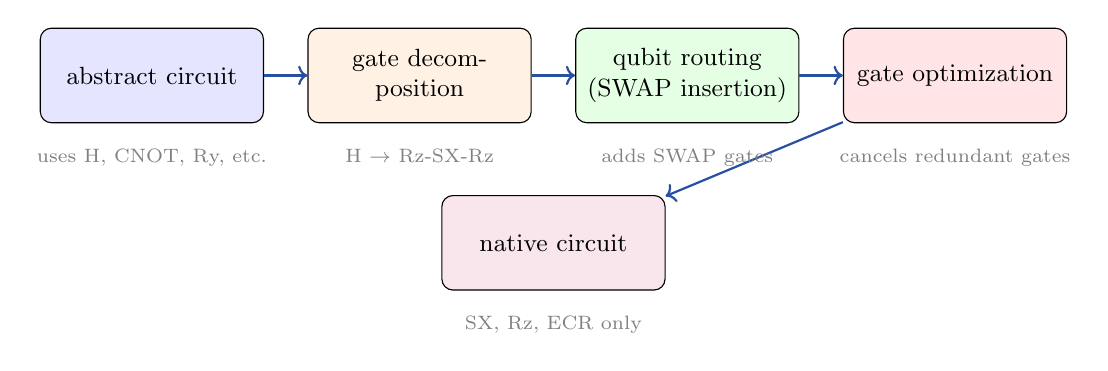
\begin{tikzpicture}[
    stage/.style={draw, rounded corners, minimum width=2.8cm, minimum height=1.2cm, font=\small, text width=2.6cm, align=center, fill=#1},
    arrow/.style={->, thick, circuitblue},
    scale=0.85
]
\node[stage=blue!10] (abstract) at (0, 0) {abstract circuit};
\node[stage=orange!10] (decomp) at (4, 0) {gate decomposition};
\node[stage=green!10] (routing) at (8, 0) {qubit routing (SWAP insertion)};
\node[stage=red!10] (opt) at (12, 0) {gate optimization};
\node[stage=purple!10] (native) at (6, -2.5) {native circuit};

\draw[arrow] (abstract) -- (decomp);
\draw[arrow] (decomp) -- (routing);
\draw[arrow] (routing) -- (opt);
\draw[arrow] (opt) -- (native);

% annotations
\node[below=0.3cm, font=\scriptsize, gray] at (0, -0.6) {uses H, CNOT, Ry, etc.};
\node[below=0.3cm, font=\scriptsize, gray] at (4, -0.6) {H $\to$ Rz-SX-Rz};
\node[below=0.3cm, font=\scriptsize, gray] at (8, -0.6) {adds SWAP gates};
\node[below=0.3cm, font=\scriptsize, gray] at (12, -0.6) {cancels redundant gates};
\node[below=0.3cm, font=\scriptsize, gray] at (6, -3.1) {SX, Rz, ECR only};
\end{tikzpicture}
\end{center}

\subsection{Transpilation Stages in Detail}

\textbf{stage 1: unrolling and decomposition.} every gate in ur circuit is decomposed into the native gate set. a hadamard becomes $R_z$-SX-$R_z$, a $R_y(\theta)$ becomes $R_z$-SX-$R_z$ combinations, a CNOT becomes an ECR with corrections.

\textbf{stage 2: routing.} the transpiler maps logical qubits to physical qubits and inserts SWAP gates wherever the circuit requires a two-qubit gate between non-adjacent qubits. this is the stage that can massively increase circuit depth. the routing problem is NP-hard in general, but good heuristics (like SABRE --- SWAP-based bidirectional heuristic search) work well in practice.

\textbf{stage 3: optimization.} after routing, the circuit often has redundant gates that can be canceled or simplified:
\begin{itemize}[leftmargin=*]
    \item adjacent inverse gates cancel: $R_z(\theta) R_z(-\theta) = I$
    \item adjacent same-axis rotations merge: $R_z(\alpha) R_z(\beta) = R_z(\alpha + \beta)$
    \item template matching: known circuit identities r applied to simplify subcircuits
    \item two-qubit gate cancellation: back-to-back CNOTs cancel
\end{itemize}

\subsection{Optimization Levels in Qiskit}

Qiskit's \texttt{transpile} function supports four optimization levels:

\begin{center}
\renewcommand{\arraystretch}{1.3}
\begin{tabular}{|c|p{8cm}|c|}
\hline
\textbf{Level} & \textbf{What It Does} & \textbf{Speed} \\
\hline
0 & minimal: just decompose to native gates and do basic routing. no optimization. & fastest \\
\hline
1 & light optimization: merge adjacent rotations, cancel inverse gates, basic layout selection. this is the default. & fast \\
\hline
2 & medium: adds more aggressive gate cancellation, template matching, commutation analysis. & moderate \\
\hline
3 & heavy: tries multiple initial layouts, uses the best one. most aggressive optimization including two-qubit block consolidation and resynthesis. & slowest \\
\hline
\end{tabular}
\end{center}

\begin{keypoint}
for QML, always use optimization level 3 for production runs. the extra compilation time (seconds to minutes) is negligible compared to the execution time, and it can reduce ur two-qubit gate count by 20--50\%. for rapid prototyping during development, level 1 is fine.
\end{keypoint}

\subsection{Impact on Circuit Depth: Before vs After}

lets see how transpilation affects a simple QML circuit.

\begin{example}[Transpilation Impact]
consider a 4-qubit, 2-layer ansatz with all-to-all CNOT connectivity on a linear chain topology ($q_0 - q_1 - q_2 - q_3$):

\textbf{before transpilation:}
\begin{itemize}[leftmargin=*]
    \item 4 qubits, 2 layers
    \item each layer: 4 $R_y$ gates + 6 CNOT gates (all pairs)
    \item total: 8 $R_y$ + 12 CNOT = 20 abstract gates
    \item abstract depth: $\sim$8
\end{itemize}

\textbf{after transpilation (level 3, linear chain):}
\begin{itemize}[leftmargin=*]
    \item non-adjacent CNOTs ($q_0$-$q_2$, $q_0$-$q_3$, $q_1$-$q_3$) need SWAP routing
    \item 6 CNOTs become $\sim$12--18 native ECR gates (due to SWAPs)
    \item single-qubit gates: $\sim$30--40 (SX + $R_z$)
    \item native depth: $\sim$25--35
\end{itemize}

the depth increased by $\sim$3--4x due to SWAP routing. this is why hardware-efficient ansatze that only use nearest-neighbor connections r so important.
\end{example}

\begin{center}
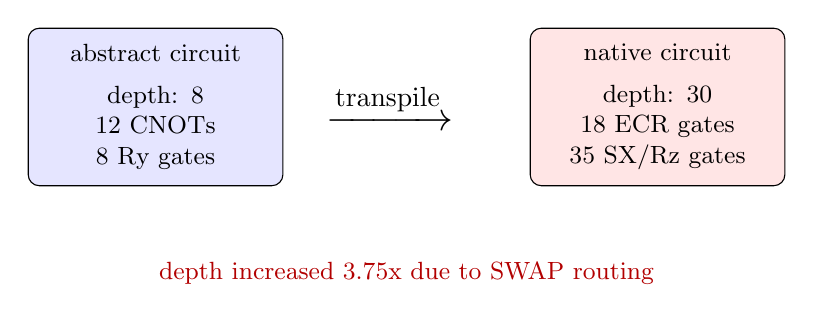
\begin{tikzpicture}[
    box/.style={draw, rounded corners, minimum width=3cm, minimum height=2cm, font=\small, text width=3cm, align=center},
    scale=0.85
]
\node[box, fill=blue!10] (before) at (0, 0) {abstract circuit\\[4pt] depth: 8\\12 CNOTs\\8 Ry gates};
\node[font=\Large] at (3.5, 0) {$\xrightarrow{\text{transpile}}$};
\node[box, fill=red!10] (after) at (7.5, 0) {native circuit\\[4pt] depth: 30\\18 ECR gates\\35 SX/Rz gates};

\node[below=1cm, font=\small, text=red!70!black] at (3.75, -1) {depth increased 3.75x due to SWAP routing};
\end{tikzpicture}
\end{center}

%% ========================================================
\section{SWAP Networks for Connectivity Constraints}
%% ========================================================

when ur circuit requires entangling gates between non-adjacent qubits, the transpiler inserts SWAP gates to ``move'' qubit states to adjacent positions. understanding the SWAP cost for different topologies helps u design better ansatze.

\subsection{SWAP Cost by Topology}

for a circuit that needs all-to-all connectivity on $n$ qubits:

\begin{center}
\renewcommand{\arraystretch}{1.3}
\begin{tabular}{|l|c|c|}
\hline
\textbf{Topology} & \textbf{Max SWAPs per 2Q Gate} & \textbf{Overhead for All-to-All} \\
\hline
all-to-all (ions) & 0 & none \\
\hline
fully connected & 0 & none \\
\hline
square grid ($\sqrt{n} \times \sqrt{n}$) & $O(\sqrt{n})$ & $O(n^{3/2})$ \\
\hline
heavy-hex & $O(\sqrt{n})$ & $O(n^{3/2})$ \\
\hline
linear chain & $O(n)$ & $O(n^2)$ \\
\hline
\end{tabular}
\end{center}

\subsection{Odd-Even SWAP Network}

a common pattern for implementing all-to-all connectivity on a linear chain is the odd-even transposition sort. after $n$ rounds of alternating odd and even pair SWAPs, any permutation can be achieved:

\begin{center}
\begin{quantikz}
\lstick{$q_0$} & \swap{1} & \qw & \swap{1} & \qw & \swap{1} & \qw \\
\lstick{$q_1$} & \targX{} & \swap{1} & \targX{} & \swap{1} & \targX{} & \qw \\
\lstick{$q_2$} & \qw & \targX{} & \swap{1} & \targX{} & \qw & \qw \\
\lstick{$q_3$} & \qw & \qw & \targX{} & \qw & \qw & \qw
\end{quantikz}
\end{center}

after these SWAP layers, all qubit states have been permuted such that non-adjacent pairs become adjacent at some point during the network. u can interleave ur entangling gates with the SWAPs.

\subsection{Linear SWAP Strategy}

an alternative is the ``linear reversal'' strategy: repeatedly SWAP adjacent pairs to shift qubit states along the chain. to bring $q_0$ next to $q_3$ on a 4-qubit linear chain, u SWAP $q_0$ through $q_1$, then through $q_2$:

depth cost: $n - 1$ SWAP layers to bring the farthest qubits together. each SWAP layer adds depth 3 (in CNOT) or depth 1 (in native SWAP gates if available).

%% ========================================================
\section{RealAmplitudes Ansatz}
%% ========================================================

RealAmplitudes is one of the simplest and most commonly used hardware-efficient ansatze in Qiskit. its a good starting point for most QML tasks.

\subsection{Structure}

\begin{definition}[RealAmplitudes Ansatz]
the RealAmplitudes ansatz consists of alternating layers of:
\begin{enumerate}[label=(\arabic*)]
    \item $R_y(\theta)$ rotations on each qubit
    \item CNOT entangling gates between pairs of qubits (configurable: linear, full, circular, etc.)
\end{enumerate}
the name comes from the fact that $R_y$ rotations and CNOTs preserve real amplitudes --- if u start from $\ket{0}^{\otimes n}$ (which has real amplitudes), the output state always has real amplitudes. the state can be written as:
\[
\ket{\psi(\theta)} = \prod_{l=1}^{L} \left[\text{Ent}_l \cdot \bigotimes_{i=0}^{n-1} R_y(\theta_i^{(l)})\right] \cdot \bigotimes_{i=0}^{n-1} R_y(\theta_i^{(0)}) \ket{0}^{\otimes n}
\]
\end{definition}

\subsection{Circuit Diagram}

3-qubit RealAmplitudes with 2 layers and linear entanglement:

\begin{center}
\begin{quantikz}
\lstick{$q_0$} & \gate{R_y(\theta_0)} & \ctrl{1} & \qw & \gate{R_y(\theta_3)} & \ctrl{1} & \qw & \gate{R_y(\theta_6)} & \qw \\
\lstick{$q_1$} & \gate{R_y(\theta_1)} & \targ{} & \ctrl{1} & \gate{R_y(\theta_4)} & \targ{} & \ctrl{1} & \gate{R_y(\theta_7)} & \qw \\
\lstick{$q_2$} & \gate{R_y(\theta_2)} & \qw & \targ{} & \gate{R_y(\theta_5)} & \qw & \targ{} & \gate{R_y(\theta_8)} & \qw
\end{quantikz}
\end{center}

4-qubit RealAmplitudes with 2 layers and linear entanglement:

\begin{center}
\begin{quantikz}
\lstick{$q_0$} & \gate{R_y(\theta_0)} & \ctrl{1} & \qw & \qw & \gate{R_y(\theta_4)} & \ctrl{1} & \qw & \qw & \gate{R_y(\theta_8)} & \qw \\
\lstick{$q_1$} & \gate{R_y(\theta_1)} & \targ{} & \ctrl{1} & \qw & \gate{R_y(\theta_5)} & \targ{} & \ctrl{1} & \qw & \gate{R_y(\theta_9)} & \qw \\
\lstick{$q_2$} & \gate{R_y(\theta_2)} & \qw & \targ{} & \ctrl{1} & \gate{R_y(\theta_6)} & \qw & \targ{} & \ctrl{1} & \gate{R_y(\theta_{10})} & \qw \\
\lstick{$q_3$} & \gate{R_y(\theta_3)} & \qw & \qw & \targ{} & \gate{R_y(\theta_7)} & \qw & \qw & \targ{} & \gate{R_y(\theta_{11})} & \qw
\end{quantikz}
\end{center}

\subsection{Parameter Count}

for $n$ qubits and $L$ entangling layers:
\[
N_{\text{params}} = n(L + 1)
\]
(each of the $L+1$ rotation layers has $n$ parameters).

for the 4-qubit, 2-layer example above: $4 \times 3 = 12$ parameters.

\subsection{Gate Count}

\begin{itemize}[leftmargin=*]
    \item single-qubit gates: $n(L+1)$ $R_y$ gates
    \item two-qubit gates: $L(n-1)$ CNOTs (for linear entanglement)
    \item total depth: $\sim 3L + 1$ (each entangling layer has depth $\sim$2--3)
\end{itemize}

\subsection{When to Use RealAmplitudes}

\begin{itemize}[leftmargin=*]
    \item ur problem has real-valued wave functions (many optimization problems)
    \item u want the simplest possible ansatz as a baseline
    \item ur hardware budget is very tight and u need minimal gate count
    \item ur training data is real-valued and u dont expect complex phases to help
\end{itemize}

\begin{intuition}
RealAmplitudes is the ``linear regression'' of quantum ansatze --- simple, interpretable, and a good first thing to try. if it doesnt work, move to smtg more expressive. if it does work, u probably dont need smtg more complex.
\end{intuition}

%% ========================================================
\section{EfficientSU2 Ansatz}
%% ========================================================

EfficientSU2 is a more expressive hardware-efficient ansatz that can produce arbitrary single-qubit states (not just real amplitudes).

\subsection{Structure}

\begin{definition}[EfficientSU2 Ansatz]
the EfficientSU2 ansatz consists of alternating layers of:
\begin{enumerate}[label=(\arabic*)]
    \item two single-qubit rotations per qubit (by default $R_y(\theta)$ followed by $R_z(\phi)$) --- this gives full SU(2) coverage on each qubit
    \item CNOT entangling gates (configurable connectivity)
\end{enumerate}
the state is:
\[
\ket{\psi(\theta, \phi)} = \prod_{l=1}^{L} \left[\text{Ent}_l \cdot \bigotimes_{i=0}^{n-1} R_z(\phi_i^{(l)}) R_y(\theta_i^{(l)})\right] \cdot \bigotimes_{i=0}^{n-1} R_z(\phi_i^{(0)}) R_y(\theta_i^{(0)}) \ket{0}^{\otimes n}
\]
\end{definition}

\subsection{Circuit Diagram}

3-qubit EfficientSU2 with 2 layers and linear entanglement:

\begin{center}
\begin{quantikz}
\lstick{$q_0$} & \gate{R_y} & \gate{R_z} & \ctrl{1} & \qw & \gate{R_y} & \gate{R_z} & \ctrl{1} & \qw & \gate{R_y} & \gate{R_z} & \qw \\
\lstick{$q_1$} & \gate{R_y} & \gate{R_z} & \targ{} & \ctrl{1} & \gate{R_y} & \gate{R_z} & \targ{} & \ctrl{1} & \gate{R_y} & \gate{R_z} & \qw \\
\lstick{$q_2$} & \gate{R_y} & \gate{R_z} & \qw & \targ{} & \gate{R_y} & \gate{R_z} & \qw & \targ{} & \gate{R_y} & \gate{R_z} & \qw
\end{quantikz}
\end{center}

4-qubit EfficientSU2 with 1 layer and linear entanglement:

\begin{center}
\begin{quantikz}
\lstick{$q_0$} & \gate{R_y} & \gate{R_z} & \ctrl{1} & \qw & \qw & \gate{R_y} & \gate{R_z} & \qw \\
\lstick{$q_1$} & \gate{R_y} & \gate{R_z} & \targ{} & \ctrl{1} & \qw & \gate{R_y} & \gate{R_z} & \qw \\
\lstick{$q_2$} & \gate{R_y} & \gate{R_z} & \qw & \targ{} & \ctrl{1} & \gate{R_y} & \gate{R_z} & \qw \\
\lstick{$q_3$} & \gate{R_y} & \gate{R_z} & \qw & \qw & \targ{} & \gate{R_y} & \gate{R_z} & \qw
\end{quantikz}
\end{center}

\subsection{Parameter Count}

for $n$ qubits and $L$ entangling layers:
\[
N_{\text{params}} = 2n(L + 1)
\]
(each rotation layer has $2n$ parameters --- one $R_y$ and one $R_z$ per qubit).

for 4 qubits, 2 layers: $2 \times 4 \times 3 = 24$ parameters (double that of RealAmplitudes).

\subsection{Comparison with RealAmplitudes}

\begin{center}
\renewcommand{\arraystretch}{1.3}
\begin{tabular}{|l|c|c|}
\hline
\textbf{Property} & \textbf{RealAmplitudes} & \textbf{EfficientSU2} \\
\hline
rotations per qubit per layer & 1 ($R_y$) & 2 ($R_y + R_z$) \\
\hline
parameters ($n$ qubits, $L$ layers) & $n(L+1)$ & $2n(L+1)$ \\
\hline
can produce complex amplitudes & no & yes \\
\hline
single-qubit gate cost & lower & higher ($\sim$2x) \\
\hline
expressibility & lower & higher \\
\hline
training difficulty & easier & harder (more parameters) \\
\hline
typical use & real-valued problems & general QML \\
\hline
\end{tabular}
\end{center}

\begin{keypoint}
EfficientSU2 has twice the parameters of RealAmplitudes for the same depth and qubit count. this means more expressiveness but also harder training (more parameters to optimize). in practice, start with RealAmplitudes. if the model isnt expressive enough, switch to EfficientSU2 before increasing the number of layers.
\end{keypoint}

%% ========================================================
\section{TwoLocal Ansatz}
%% ========================================================

TwoLocal is the general framework that both RealAmplitudes and EfficientSU2 r special cases of. it gives u full control over the ansatz structure.

\subsection{Configuration}

\begin{definition}[TwoLocal Ansatz]
a TwoLocal ansatz is specified by:
\begin{enumerate}[label=(\arabic*)]
    \item \textbf{rotation blocks}: which single-qubit gates to use (e.g., [$R_y$], [$R_y$, $R_z$], [$R_x$, $R_y$, $R_z$])
    \item \textbf{entanglement blocks}: which two-qubit gates to use (e.g., CNOT, CZ, $R_{zz}$)
    \item \textbf{entanglement pattern}: which qubit pairs to entangle (linear, full, circular, pairwise, custom list)
    \item \textbf{number of repetitions}: how many layers $L$
    \item \textbf{skip final rotation}: whether to include the last rotation layer
\end{enumerate}
\end{definition}

\begin{example}[Custom TwoLocal]
a TwoLocal with rotation blocks $[R_x, R_z]$, entanglement block CZ, circular entanglement, 2 repetitions on 3 qubits produces:

\begin{center}
\begin{quantikz}
\lstick{$q_0$} & \gate{R_x} & \gate{R_z} & \ctrl{1} & \qw & \ctrl{2} & \gate{R_x} & \gate{R_z} & \ctrl{1} & \qw & \ctrl{2} & \gate{R_x} & \gate{R_z} & \qw \\
\lstick{$q_1$} & \gate{R_x} & \gate{R_z} & \control{} & \ctrl{1} & \qw & \gate{R_x} & \gate{R_z} & \control{} & \ctrl{1} & \qw & \gate{R_x} & \gate{R_z} & \qw \\
\lstick{$q_2$} & \gate{R_x} & \gate{R_z} & \qw & \control{} & \control{} & \gate{R_x} & \gate{R_z} & \qw & \control{} & \control{} & \gate{R_x} & \gate{R_z} & \qw
\end{quantikz}
\end{center}
(using CZ gates, shown as controlled-Z with control dots on both qubits)
\end{example}

the key insight: RealAmplitudes is just TwoLocal with rotation\_blocks=$[R_y]$ and entanglement\_blocks=$[\text{CNOT}]$. EfficientSU2 is TwoLocal with rotation\_blocks=$[R_y, R_z]$ and entanglement\_blocks=$[\text{CNOT}]$.

%% ========================================================
\section{Hardware-Efficient vs Problem-Inspired Ansatze}
%% ========================================================

theres an important distinction between hardware-efficient ansatze (designed for the hardware) and problem-inspired ansatze (designed for the problem). lets compare.

\subsection{The Tradeoff}

\begin{center}
\renewcommand{\arraystretch}{1.4}
\begin{tabular}{|l|c|c|}
\hline
\textbf{Property} & \textbf{Hardware-Efficient} & \textbf{Problem-Inspired} \\
\hline
design principle & minimize hardware cost & encode problem structure \\
\hline
examples & RealAmplitudes, EfficientSU2 & UCCSD, QAOA, HVA \\
\hline
native gates? & yes (by construction) & usually no \\
\hline
respects topology? & yes (by construction) & usually no \\
\hline
circuit depth (before transpile) & low & moderate to high \\
\hline
circuit depth (after transpile) & low (minimal change) & high (SWAP overhead) \\
\hline
expressibility & generic, untargeted & targeted to problem \\
\hline
trainability & often barren plateaus & better gradients \\
\hline
physical motivation & none & symmetries, conservation laws \\
\hline
parameter efficiency & low (many params, generic) & high (fewer params, targeted) \\
\hline
\end{tabular}
\end{center}

\begin{keypoint}
the big surprise from the literature (mcclean et al.\ 2018): randomly structured hardware-efficient ansatze tend to have barren plateaus --- the gradient vanishes exponentially with the number of qubits. problem-inspired ansatze often avoid this bcs they start with a structure thats already close to the solution.

but on noisy hardware, the problem-inspired ansatz might be too deep to run, while the hardware-efficient one actually executes. so the practical choice depends on ur specific hardware noise budget.
\end{keypoint}

\subsection{When to Use Which}

\textbf{use hardware-efficient when:}
\begin{itemize}[leftmargin=*]
    \item ur working on NISQ hardware with tight noise budgets
    \item u dont have strong prior knowledge about the problem structure
    \item ur problem is a generic classification or regression task
    \item u need fast iteration (short circuits = fast execution)
\end{itemize}

\textbf{use problem-inspired when:}
\begin{itemize}[leftmargin=*]
    \item the problem has known symmetries (e.g., particle number conservation in chemistry)
    \item the hardware can support the required depth (e.g., trapped ions, or error-mitigated superconducting)
    \item u need good trainability and dont want to fight barren plateaus
    \item accuracy matters more than speed
\end{itemize}

%% ========================================================
\section{Reducing Two-Qubit Gate Count}
%% ========================================================

since two-qubit gates r $\sim$10x noisier than single-qubit gates, reducing their count is the most impactful optimization u can make.

\subsection{Gate Cancellation}

the simplest technique: adjacent inverse gates cancel.
\[
\text{CNOT}_{01} \cdot \text{CNOT}_{01} = I
\]

this happens surprisingly often when circuits r composed from layers --- the last CNOT of one layer and the first CNOT of the next might cancel.

\subsection{Template Matching}

certain circuit patterns can be replaced by shorter equivalents:

\begin{example}
the ``CNOT cascade'' identity:
\begin{center}
\begin{quantikz}
\lstick{$q_0$} & \ctrl{1} & \qw & \qw \\
\lstick{$q_1$} & \targ{} & \ctrl{1} & \qw \\
\lstick{$q_2$} & \qw & \targ{} & \qw
\end{quantikz}
$\quad \neq \quad$
\begin{quantikz}
\lstick{$q_0$} & \ctrl{2} & \ctrl{1} & \qw \\
\lstick{$q_1$} & \qw & \targ{} & \qw \\
\lstick{$q_2$} & \targ{} & \qw & \qw
\end{quantikz}
\end{center}
(these r different circuits --- template matching finds exact equivalences)

a real template: two CNOTs with a rotation between them can sometimes be simplified:
\[
\text{CNOT}_{01} \cdot (I \otimes R_z(\theta)) \cdot \text{CNOT}_{01} = R_{zz}(\theta) \otimes I
\]
(up to single-qubit corrections). this reduces 2 CNOTs to the equivalent of $\sim$1 CNOT.
\end{example}

\subsection{Commutation Analysis}

gates that commute can be reordered to enable cancellations:
\begin{itemize}[leftmargin=*]
    \item $R_z$ commutes with CNOT (on control qubit): $(\text{CNOT}_{01})(R_z(\theta) \otimes I) = (R_z(\theta) \otimes I)(\text{CNOT}_{01})$
    \item CZ is symmetric: $\text{CZ}_{01} = \text{CZ}_{10}$
    \item commuting gates through each other can bring adjacent gates together for cancellation
\end{itemize}

\subsection{Two-Qubit Block Consolidation}

Qiskit optimization level 3 does smtg clever: it identifies blocks of consecutive two-qubit gates, computes the unitary of the entire block (a $4 \times 4$ matrix), and resynthesizes it using the minimum number of native two-qubit gates via KAK decomposition.

for example, a sequence of 4 CNOTs between qubits 0 and 1 might consolidate to just 1 or 2 CNOTs plus single-qubit gates, bcs the combined unitary might not require all 3 CNOTs that a general SU(4) needs.

%% ========================================================
\section{QAOA as a Hardware-Aware Ansatz}
%% ========================================================

the quantum approximate optimization algorithm (QAOA) is interesting bcs it sits between hardware-efficient and problem-inspired. lets see why.

\subsection{QAOA Structure}

recall from earlier lectures that QAOA for a cost function $C$ uses the ansatz:
\[
\ket{\gamma, \beta} = \prod_{p=1}^{P} e^{-i\beta_p \hat{B}} e^{-i\gamma_p \hat{C}} \ket{+}^{\otimes n}
\]
where $\hat{B} = \sum_i X_i$ (mixer) and $\hat{C}$ encodes the problem.

for a MaxCut problem on graph $G = (V, E)$:
\[
\hat{C} = \sum_{(i,j) \in E} \frac{1}{2}(I - Z_i Z_j)
\]

the cost unitary decomposes as:
\[
e^{-i\gamma \hat{C}} = \prod_{(i,j) \in E} e^{-i\gamma \frac{1}{2}(I - Z_i Z_j)} = \prod_{(i,j) \in E} R_{ZZ}(\gamma)_{ij}
\]

each $R_{ZZ}(\gamma)$ requires one CNOT (or native two-qubit gate) plus single-qubit rotations.

\subsection{Why QAOA Can Be Hardware-Efficient}

heres the key insight: if the problem graph $G$ matches the hardware topology, then QAOA is automatically hardware-efficient.

\begin{example}
consider MaxCut on a graph thats isomorphic to the hardware connectivity graph (e.g., a heavy-hex graph on IBM hardware). then every $R_{ZZ}$ gate in the cost unitary corresponds to a physically connected qubit pair --- no SWAP routing needed. the circuit depth per QAOA layer is $O(1)$ (since gates on different edges can be parallelized).
\end{example}

\begin{keypoint}
for optimization problems where the problem graph naturally matches the hardware topology, QAOA is both problem-inspired AND hardware-efficient. this is the best of both worlds. in general, QAOA's hardware cost scales with the ``distance'' between the problem graph and the hardware graph.
\end{keypoint}

the QAOA circuit for MaxCut on 4 qubits with linear connectivity ($q_0$-$q_1$-$q_2$-$q_3$):

\begin{center}
\begin{quantikz}
\lstick{$q_0$} & \gate{H} & \ctrl{1} & \qw & \qw & \gate{R_x(\beta_1)} & \ctrl{1} & \qw & \qw & \gate{R_x(\beta_2)} & \qw \\
\lstick{$q_1$} & \gate{H} & \gate{R_{zz}(\gamma_1)} & \ctrl{1} & \qw & \gate{R_x(\beta_1)} & \gate{R_{zz}(\gamma_2)} & \ctrl{1} & \qw & \gate{R_x(\beta_2)} & \qw \\
\lstick{$q_2$} & \gate{H} & \qw & \gate{R_{zz}(\gamma_1)} & \ctrl{1} & \gate{R_x(\beta_1)} & \qw & \gate{R_{zz}(\gamma_2)} & \ctrl{1} & \gate{R_x(\beta_2)} & \qw \\
\lstick{$q_3$} & \gate{H} & \qw & \qw & \gate{R_{zz}(\gamma_1)} & \gate{R_x(\beta_1)} & \qw & \qw & \gate{R_{zz}(\gamma_2)} & \gate{R_x(\beta_2)} & \qw
\end{quantikz}
\end{center}

(here $R_{zz}(\gamma)$ between control and target is shorthand for the ZZ interaction implemented via CNOT-$R_z$-CNOT)

%% ========================================================
\section{Practical Ansatz Design Checklist}
%% ========================================================

when designing an ansatz for a specific hardware backend, follow this checklist:

\subsection{Step 1: Know Ur Hardware}

\begin{enumerate}[label=\arabic*.]
    \item wt is the native gate set? (check backend configuration)
    \item wt is the connectivity map? (check coupling map)
    \item wt r the current gate errors? (check calibration data)
    \item wt r the coherence times? (check $T_1$, $T_2$ per qubit)
    \item which qubits r best right now? (check latest calibration)
\end{enumerate}

\subsection{Step 2: Compute Ur Noise Budget}

estimate the maximum circuit depth:
\[
D_{\max} \approx \frac{-\ln(\epsilon_{\text{target}})}{n_{2Q} \cdot \epsilon_{2Q} + n_{1Q} \cdot \epsilon_{1Q}}
\]

where $\epsilon_{\text{target}}$ is ur acceptable total error (e.g., 0.3 for a QML classifier).

\begin{example}
for IBM Heron with $\epsilon_{2Q} = 0.003$, $\epsilon_{1Q} = 0.0003$, 10 qubits:
\[
D_{\max} \approx \frac{-\ln(0.3)}{9 \times 0.003 + 10 \times 0.0003} \approx \frac{1.2}{0.027 + 0.003} = \frac{1.2}{0.03} = 40 \text{ layers}
\]
so u can afford about 40 entangling layers. thats actually quite generous for a hardware-efficient ansatz.
\end{example}

\subsection{Step 3: Choose Ansatz Family}

\begin{center}
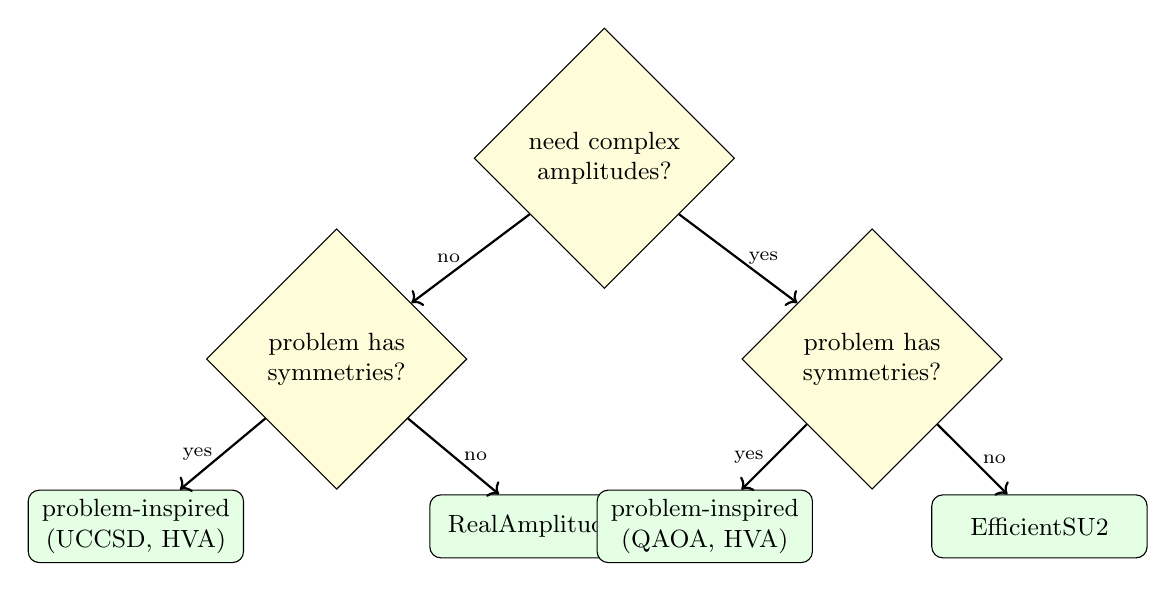
\begin{tikzpicture}[
    decision/.style={diamond, draw, fill=yellow!15, text width=2.5cm, align=center, inner sep=1pt, font=\small},
    result/.style={draw, rounded corners, fill=green!10, text width=2.5cm, align=center, font=\small, minimum height=0.8cm},
    arrow/.style={->, thick},
    scale=0.85
]
\node[decision] (q1) at (4, 6) {need complex amplitudes?};
\node[decision] (q2) at (0, 3) {problem has symmetries?};
\node[decision] (q3) at (8, 3) {problem has symmetries?};

\node[result] (r1) at (-3, 0.5) {problem-inspired (UCCSD, HVA)};
\node[result] (r2) at (3, 0.5) {RealAmplitudes};
\node[result] (r3) at (5.5, 0.5) {problem-inspired (QAOA, HVA)};
\node[result] (r4) at (10.5, 0.5) {EfficientSU2};

\draw[arrow] (q1) -- node[left, font=\scriptsize] {no} (q2);
\draw[arrow] (q1) -- node[right, font=\scriptsize] {yes} (q3);
\draw[arrow] (q2) -- node[left, font=\scriptsize] {yes} (r1);
\draw[arrow] (q2) -- node[right, font=\scriptsize] {no} (r2);
\draw[arrow] (q3) -- node[left, font=\scriptsize] {yes} (r3);
\draw[arrow] (q3) -- node[right, font=\scriptsize] {no} (r4);
\end{tikzpicture}
\end{center}

\subsection{Step 4: Configure Entanglement Pattern}

match the entanglement pattern to ur hardware:
\begin{itemize}[leftmargin=*]
    \item \textbf{linear chain topology}: use ``linear'' entanglement (neighbor pairs)
    \item \textbf{heavy-hex topology}: design custom entanglement map matching the hardware edges
    \item \textbf{all-to-all (trapped ions)}: use ``full'' entanglement for maximum expressiveness
    \item \textbf{square grid}: use ``pairwise'' entanglement alternating horizontal and vertical edges
\end{itemize}

\subsection{Step 5: Set Number of Layers}

start small and increase:
\begin{enumerate}[label=\arabic*.]
    \item start with $L = 1$ (minimal ansatz)
    \item train and evaluate. if the model underfits, increase $L$
    \item keep increasing until u hit one of: (a) good performance, (b) overfitting, (c) noise budget limit, (d) barren plateaus (gradients vanish)
    \item typical good range: $L = 2$--$6$ for current NISQ hardware
\end{enumerate}

\subsection{Step 6: Transpile and Verify}

\begin{enumerate}[label=\arabic*.]
    \item transpile ur circuit at optimization level 3
    \item check the native gate count (especially 2Q gates)
    \item verify the native depth is within ur noise budget
    \item if its too deep, reduce layers or simplify entanglement
    \item compare with a random circuit of the same structure to check for barren plateaus
\end{enumerate}

%% ========================================================
\section{The Qiskit Pass Manager}
%% ========================================================

for fine-grained control over transpilation, Qiskit provides the pass manager framework. understanding it helps u optimize beyond what the default \texttt{transpile()} function does.

\subsection{Transpilation Passes}

a ``pass'' is a single transformation applied to a circuit. passes r grouped into stages:

\begin{enumerate}[label=\arabic*.]
    \item \textbf{init stage}: high-level optimization before layout (e.g., unrolling custom gates)
    \item \textbf{layout stage}: map logical qubits to physical qubits (e.g., TrivialLayout, SabreLayout, DenseLayout)
    \item \textbf{routing stage}: insert SWAPs for non-local gates (e.g., SabreSwap, StochasticSwap)
    \item \textbf{translation stage}: convert to native gates (e.g., BasisTranslator, UnrollCustomDefinitions)
    \item \textbf{optimization stage}: reduce gate count (e.g., Optimize1qGates, CXCancellation, CommutativeCancellation)
    \item \textbf{scheduling stage}: add timing information for pulse-level execution
\end{enumerate}

\subsection{Optimization Passes in Detail}

the key optimization passes for reducing 2Q gate count:

\textbf{CXCancellation}: finds and removes adjacent CNOT pairs:
\[
\text{CNOT}_{01} \cdot \text{CNOT}_{01} \to I
\]

\textbf{CommutativeCancellation}: identifies gates that commute, reorders them, and cancels:
\[
\text{CNOT}_{01} \cdot (R_z \otimes I) \cdot \text{CNOT}_{01} \to R_{zz} \text{ equivalent}
\]

\textbf{Collect2qBlocks + ConsolidateBlocks}: groups consecutive 2Q gates into blocks, computes the unitary, and resynthesizes with minimum gates.

\textbf{TemplateOptimization}: matches known circuit identities and applies simplifications.

\begin{example}[Custom Pass Manager for QML]
a practical pass manager for QML circuits:
\begin{enumerate}[label=\arabic*.]
    \item use SabreLayout with multiple random seeds (try 20--50 layouts, keep the best)
    \item use SabreSwap for routing
    \item run Collect2qBlocks + ConsolidateBlocks to minimize 2Q gates
    \item run CommutativeCancellation
    \item run Optimize1qGatesDecomposition to merge single-qubit gates
    \item repeat optimization passes 2--3 times (each pass can enable new optimizations)
\end{enumerate}
\end{example}

%% ========================================================
\section{Circuit Depth Optimization Techniques}
%% ========================================================

beyond the transpiler, there r several techniques u can use to reduce circuit depth at the design level.

\subsection{Parallelization}

gates on non-overlapping qubits can execute simultaneously. design ur entanglement layers to maximize parallelism:

\textbf{bad (sequential):}
\[
\text{CNOT}_{01} \to \text{CNOT}_{12} \to \text{CNOT}_{23} \to \text{CNOT}_{34} \quad (\text{depth } 4)
\]

\textbf{good (parallel):}
\[
\{\text{CNOT}_{01}, \text{CNOT}_{23}\} \to \{\text{CNOT}_{12}, \text{CNOT}_{34}\} \quad (\text{depth } 2)
\]

for ``linear'' entanglement in Qiskit, the gates r automatically layered for parallelism using even/odd pairs.

\subsection{Entanglement Reduction}

instead of full (all-to-all) entanglement, use sparser patterns:

\begin{center}
\renewcommand{\arraystretch}{1.3}
\begin{tabular}{|l|c|c|c|}
\hline
\textbf{Pattern} & \textbf{2Q Gates/Layer} & \textbf{Depth/Layer} & \textbf{Expressibility} \\
\hline
linear & $n-1$ & 2 & moderate \\
\hline
circular & $n$ & 2--3 & good \\
\hline
pairwise & $\lfloor n/2 \rfloor$ & 1 & low per layer \\
\hline
full & $\binom{n}{2}$ & $n-1$ & highest \\
\hline
\end{tabular}
\end{center}

\begin{keypoint}
for QML on NISQ hardware, ``linear'' entanglement with more layers is usually better than ``full'' entanglement with fewer layers. u get similar expressiveness with much less noise bcs every gate is between adjacent qubits.
\end{keypoint}

\subsection{Layer-Wise Training}

instead of training all layers simultaneously (which can lead to barren plateaus), train one layer at a time:

\begin{enumerate}[label=\arabic*.]
    \item initialize a 1-layer ansatz, train to convergence
    \item add a second layer (initialized to identity or small random values), train
    \item repeat until adding more layers doesnt improve performance
\end{enumerate}

this doesnt reduce the final circuit depth, but it makes training much more reliable and often finds better optima.

\subsection{Parameter Sharing}

use the same parameter values across different layers:
\[
\theta_i^{(l)} = \theta_i \quad \forall l
\]

this reduces the parameter count from $n(L+1)$ to $n$ while keeping the same circuit depth. the expressiveness is reduced, but this can actually help with trainability (fewer parameters = simpler optimization landscape).

%% ========================================================
\section{Impact of Transpilation: Detailed Example}
%% ========================================================

lets work through a complete example of how transpilation transforms a QML circuit.

\subsection{The Abstract Circuit}

consider a 4-qubit EfficientSU2 ansatz with 2 layers and circular entanglement. the abstract circuit has:
\begin{itemize}[leftmargin=*]
    \item $3 \times 2 \times 4 = 24$ single-qubit rotation gates ($R_y$ and $R_z$)
    \item $2 \times 4 = 8$ CNOT gates (circular: $q_0$-$q_1$, $q_1$-$q_2$, $q_2$-$q_3$, $q_3$-$q_0$, repeated twice)
    \item abstract depth: approximately 12
\end{itemize}

\subsection{Transpilation to Linear Chain}

on a linear chain ($q_0$-$q_1$-$q_2$-$q_3$), the $q_3$-$q_0$ CNOT in each layer requires SWAP routing. lets trace through:

\textbf{layer 1 entanglement:}
\begin{itemize}[leftmargin=*]
    \item CNOT($q_0$, $q_1$): native, no change (1 ECR)
    \item CNOT($q_1$, $q_2$): native, no change (1 ECR)
    \item CNOT($q_2$, $q_3$): native, no change (1 ECR)
    \item CNOT($q_3$, $q_0$): NOT native. need to route $q_0$ state to be adjacent to $q_3$:
    \begin{itemize}
        \item SWAP($q_0$, $q_1$): 3 ECR gates
        \item SWAP($q_1$, $q_2$): 3 ECR gates
        \item CNOT($q_2$, $q_3$): 1 ECR gate
        \item (then the qubit mapping has changed --- the transpiler tracks this)
    \end{itemize}
    \item subtotal: $3 + 7 = 10$ ECR gates (vs.\ 4 ideal)
\end{itemize}

after optimization (level 3), some of these ECR gates may cancel with subsequent gates, reducing the total. typical final count: $\sim$7--8 ECR gates per layer.

\subsection{Before/After Comparison}

\begin{center}
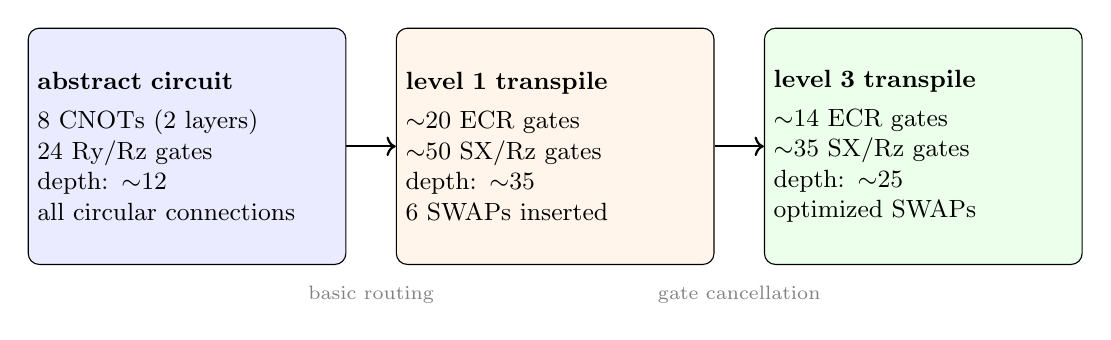
\begin{tikzpicture}[
    box/.style={draw, rounded corners, minimum width=4cm, minimum height=3cm, font=\small, text width=3.8cm, align=left},
    scale=0.85
]
\node[box, fill=blue!8] (before) at (0, 0) {
    \textbf{abstract circuit}\\[3pt]
    8 CNOTs (2 layers)\\
    24 Ry/Rz gates\\
    depth: $\sim$12\\
    all circular connections
};

\node[box, fill=orange!8] (level1) at (5.5, 0) {
    \textbf{level 1 transpile}\\[3pt]
    $\sim$20 ECR gates\\
    $\sim$50 SX/Rz gates\\
    depth: $\sim$35\\
    6 SWAPs inserted
};

\node[box, fill=green!8] (level3) at (11, 0) {
    \textbf{level 3 transpile}\\[3pt]
    $\sim$14 ECR gates\\
    $\sim$35 SX/Rz gates\\
    depth: $\sim$25\\
    optimized SWAPs
};

\draw[->, thick] (before) -- (level1);
\draw[->, thick] (level1) -- (level3);
\node[below=0.2cm, font=\scriptsize, gray] at (2.75, -1.7) {basic routing};
\node[below=0.2cm, font=\scriptsize, gray] at (8.25, -1.7) {gate cancellation};
\end{tikzpicture}
\end{center}

\begin{keypoint}
the lesson: a circuit thats designed to be hardware-efficient from the start (using only linear entanglement) would have needed only 6 ECR gates per layer (3 per layer, 2 layers) with zero SWAP overhead. thats less than half the cost of the circular version after transpilation. always design for the hardware from the beginning.
\end{keypoint}

%% ========================================================
\section{Advanced: Noise-Aware Ansatz Design}
%% ========================================================

beyond just respecting topology, u can go further and design ansatze that account for the specific noise properties of each qubit and gate.

\subsection{Qubit Quality Variation}

on a real backend, different qubits and different qubit pairs have different error rates. a noise-aware design strategy:

\begin{enumerate}[label=\arabic*.]
    \item query the backend calibration data
    \item rank qubit pairs by two-qubit gate error
    \item select a connected subgraph of the $n$ best qubits
    \item design ur entanglement pattern to use only the lowest-error qubit pairs
    \item avoid the worst qubits entirely (even if theyre physically present)
\end{enumerate}

\begin{example}
on a 127-qubit Eagle processor, the best 10-qubit subgraph might have:
\begin{itemize}[leftmargin=*]
    \item average 2Q error: 0.5\% (vs.\ 1.2\% chip average)
    \item average $T_1$: 250 $\mu$s (vs.\ 150 $\mu$s chip average)
    \item this effectively doubles ur noise budget and circuit depth limit
\end{itemize}
\end{example}

\subsection{Error-Aware Entanglement}

instead of uniform entanglement patterns, weight the entangling gates by the quality of the underlying hardware:

\begin{enumerate}[label=\arabic*.]
    \item for qubit pairs with low error: use CNOT gates (full entanglement)
    \item for qubit pairs with moderate error: use parameterized $R_{ZZ}(\theta)$ gates (can reduce entanglement strength)
    \item for qubit pairs with high error: skip the entangling gate entirely
\end{enumerate}

this creates an ansatz where the entanglement structure is adapted to the noise landscape of the specific processor.

\subsection{Dynamical Decoupling}

between gate operations, qubits idle and decohere. dynamical decoupling (DD) inserts sequences of identity-equivalent pulses during idle periods to protect against low-frequency noise:
\[
\text{DD sequence: } X - \tau - X - \tau - X - \tau - X - \tau
\]

this refocuses slow dephasing noise (similar to a spin echo). Qiskit supports automatic DD insertion during transpilation.

for QML circuits, DD is especially important when ur circuit has unbalanced depth across qubits --- some qubits might idle for many gate durations while others r busy.

%% ========================================================
\section{Summary and Design Principles}
%% ========================================================

key takeaways from this lecture:

\begin{enumerate}[label=\arabic*.]
    \item \textbf{hardware-efficient means}: native gates, native connectivity, minimal depth. design for the hardware from the start, dont rely on the transpiler to fix a bad circuit.

    \item \textbf{native gate sets matter}: use $R_z$ (virtual, zero cost) and minimize physical gates. on IBM, target SX + ECR as ur building blocks.

    \item \textbf{SWAP gates r expensive}: 3 CNOTs each, $\sim$1.5\% error. minimize non-local entanglement.

    \item \textbf{RealAmplitudes is ur starting point}: simple, $n(L+1)$ parameters, real amplitudes only. upgrade to EfficientSU2 ($2n(L+1)$ parameters) if u need more expressiveness.

    \item \textbf{transpilation at level 3}: always use it for production. it can reduce 2Q gate count by 20--50\%.

    \item \textbf{QAOA is naturally hardware-efficient} when the problem graph matches the hardware topology.

    \item \textbf{the noise budget rules everything}: compute $D_{\max}$ for ur hardware. if ur ansatz after transpilation exceeds $D_{\max}$, simplify it. no amount of error mitigation can save a circuit thats 10x too deep.

    \item \textbf{check calibration data daily}: hardware quality drifts. the best qubits today might not be the best tomorrow.

    \item \textbf{start simple, add complexity}: begin with $L=1$ RealAmplitudes on the best qubits. only add layers, parameters, or more complex ansatze when u have evidence that the simpler version isnt enough.
\end{enumerate}

\begin{keypoint}
the meta-lesson: in the NISQ era, the best QML model isnt the most theoretically powerful one --- its the one that extracts the most useful computation from a limited noise budget. hardware awareness is not an afterthought; its the first design decision.
\end{keypoint}

next lecture well apply these principles to run actual QML experiments on real hardware, dealing with all the practical issues: job management, error mitigation, result interpretation, and debugging when things go wrong (which they will).

\end{document}
